\chapter{Métodos experimentales}

\section{Escritura de guías de onda}
\begin{figure}[H]
	\centering
	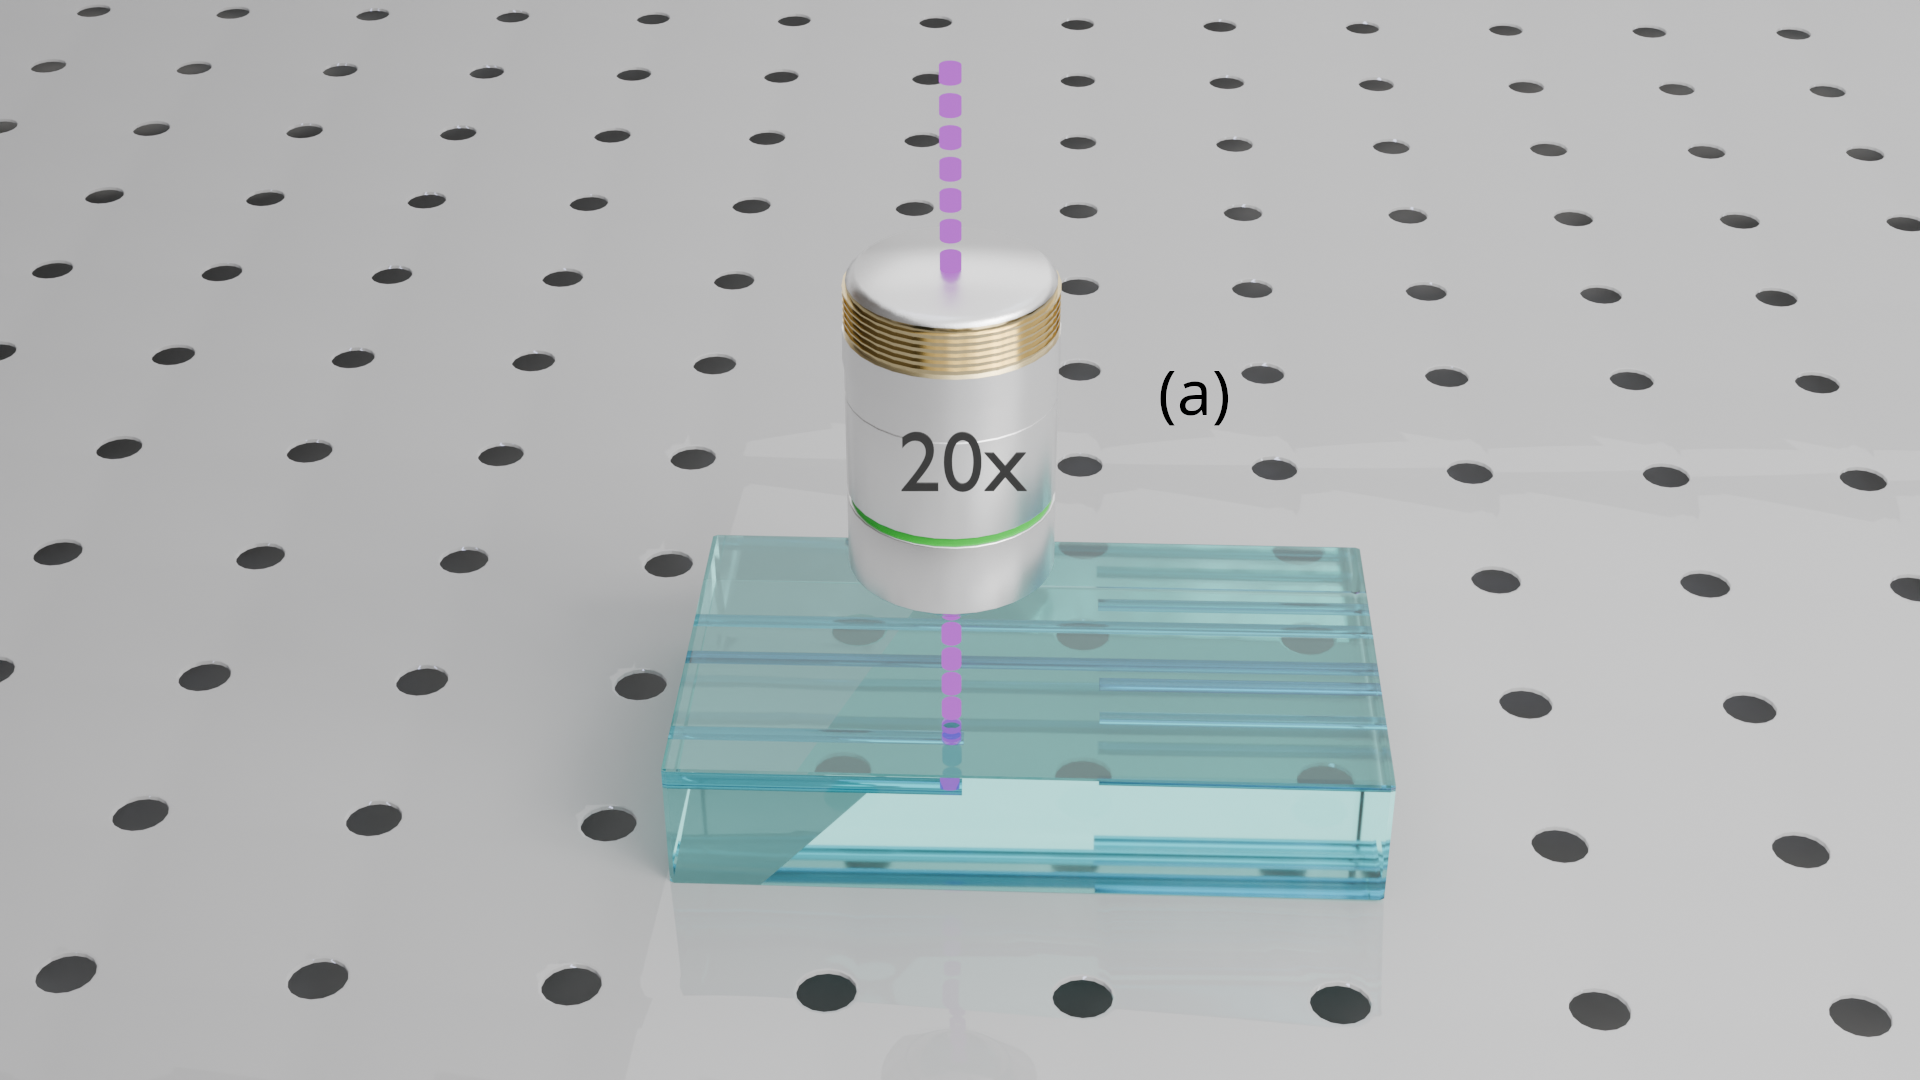
\includegraphics[width=0.6\linewidth, trim={18cm 4cm 15cm 6cm},clip]{media/fabrication}
	\caption{Escritura.}
\end{figure}

\section{Montaje de excitación láser supercontinuo}
\begin{figure}[H]
	\centering
	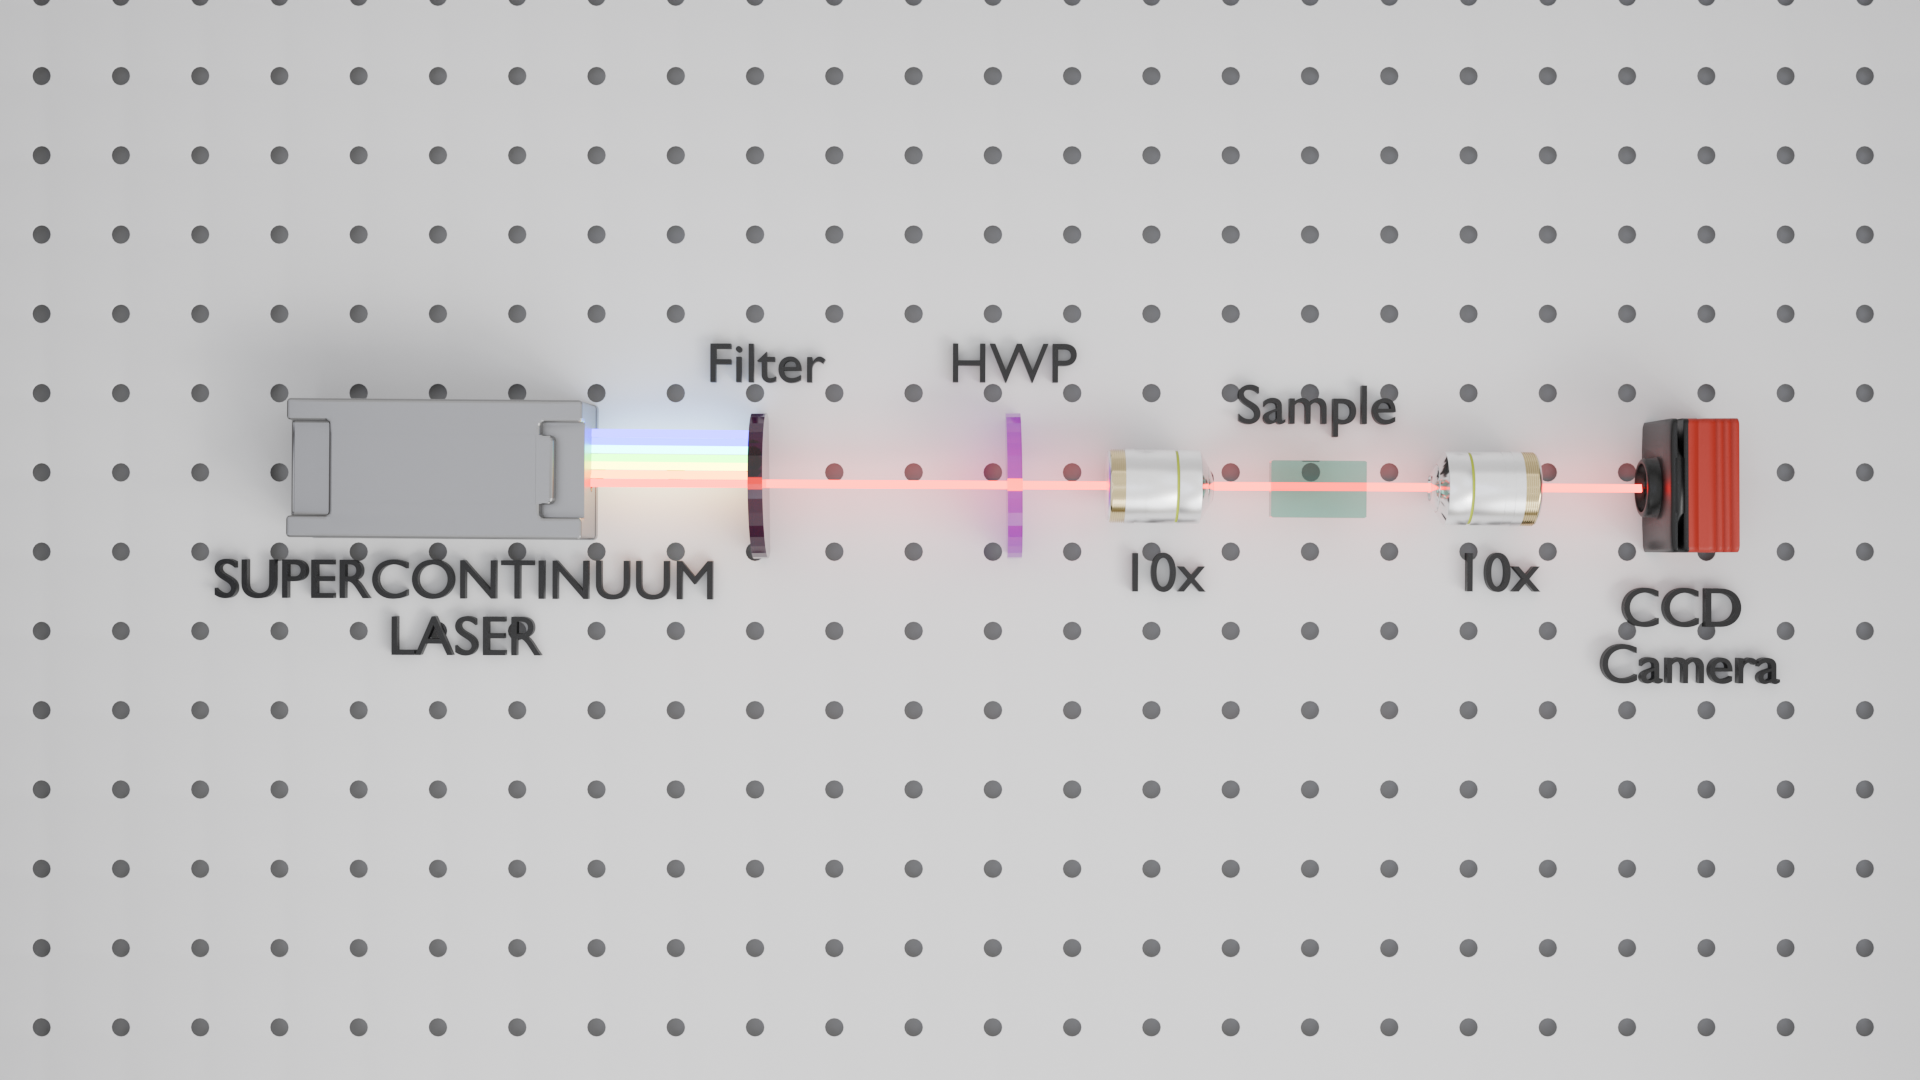
\includegraphics[width=\linewidth, trim={5cm 9cm 3cm 7cm},clip]{media/SC_setup}
	\caption{Montaje SC.}
\end{figure}
\newpage
\section{Montaje de modulación espacial de luz}

Para usar condiciones iniciales distintas a una gaussiana se hace necesario incorporar métodos de modulación espacial de luz. En esta tesis se utilizó una técnica conocida como 

\subsection{Etapa premodulación}
	El modulador espacial de luz utilizado es un HOLOEYE PLUTO-NIR SLM -  Reflective LCOS, cuya respuesta óptica ocurre con polarización paralela al plano de la mesa óptica. Se utiliza un retardador de media onda ($\lambda/2$) seguido de un polarizador de atenuación 10000:1 con el objetivo de que la polarización de la luz láser coincida con la de la respuesta del SLM. Posteriormente se magnifica y se colima el haz para que abarque todo el área de pixeles disponible.
\subsection{Etapa de modulación}
	Una rejilla de difracción que maximiza la potencia del primer orden de difracción es utilizada. Para modular en amplitud se debe multiplicar la rejilla por la máscara de amplitud deseada, mientras que para modular en fase basta con sumar el nivel de gris correspondiente a la fase deseada. FIGURA
\subsection{Etapa de acoplamiento}
\subsection{Etapa de captura en cámara}

\subsection{Circuito óptico}
\begin{figure}[H]
	\centering
	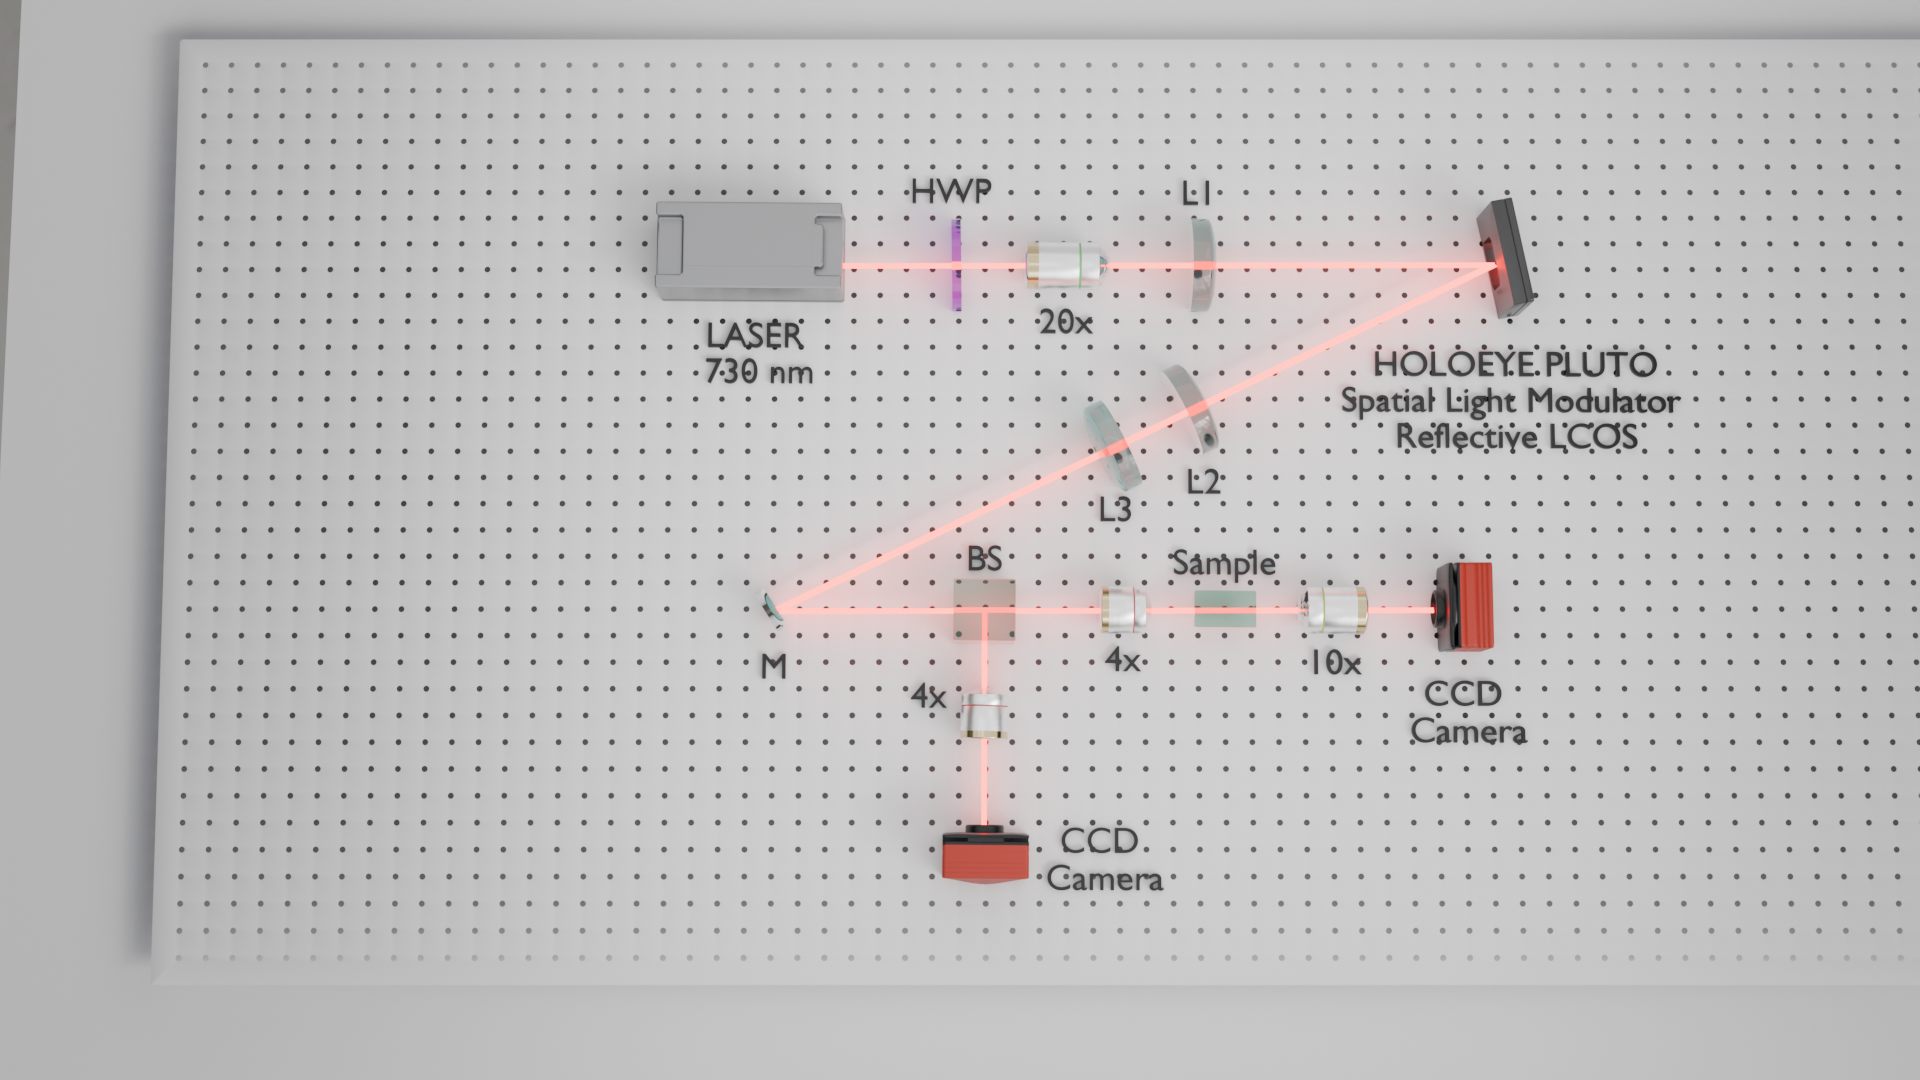
\includegraphics[width=\linewidth, trim={21cm 5cm 7cm 5cm},clip]{media/SLM_setup}
	\caption{Montaje SLM.}
\end{figure}
\section{Análisis de imágenes}

